\chapter{Implementierung}
\thispagestyle{fancy}

Als Basis der Implementierung diente das tempoGAN nach \citet{xie2018tempoGAN}. Der Unterschied zu dem tempoGAN KI-Modell bestand in der Wahl der Fields, die diese Arbeit für das Training nutze. Anstatt das Velocity Field zu nutzen, kam das Temperature Field zum Einsatz. Dieses hat ebenso wie das Velocity Field eine physikalische Grundlage innerhalb der Simulation, benötigte jedoch weniger Speicherplatz. Ebenso waren beide neuronalen Netze mit weniger Convolutional Layer aufgebaut. Diese und weitere Unterschiede zu tempoGAN werden in den folgenden Abschnitten näher betrachtet.

\section{Setup}
Das Experiment wurde auf einer von Mackevision zur Verfügung gestellten Workstation durchgeführt. Sie bestand unter anderem aus dem Intel Prozessor E5-2630 mit sechs Kernen, der Grundtaktfrequenz 2,30 GHz und einer einzelnen NVIDIA RTX 3060 Ti mit 8 Gigabyte VRAM. Die Speicherung der Daten erfolgte auf dem firmeninternen Server. Als Betriebssystem diente Windows 10.


\section{Datenerhebung}
Ein grundsätzlicher Unterschied zur tempoGAN-Implementierung war die Erzeugung des Datensatzes von Simulationsdaten. Dort wurden die Simulationen innerhalb der Software \textit{Mantaflow} \parencite{mantaflow} erstellt. Ebenso setzt Mantaflow auf ein selbst entwickeltes Dateiformat der Endung \textit{.uni}, um Raster- und Partikeldaten zu speichern \parencite[]{thuerey-group-no-date}. Houdini hingegen arbeitet nicht mit einer Mantaflow-Implementierung und um zu testen, ob ein KI-Modell mit den Daten der gängigen Programme im VFX Bereich trainiert werden konnte, wurde auf die Nutzung von Mantaflow verzichtet. 
Als Trainingsdaten dienten die wie im Methodik-Abschnitt erzeugten Rauchsimulationen verwendet. Hier lag ein weiterer Unterschied zur tempoGAN-Implementierung. Die Forscher trainierten das KI-Modell mit den Density und Velocity Fields ihrer Simulationen. Wurde jedoch auf den Export des Velocity Fields verzichtet und stattdessen das Temperature Field genutzt, ließen sich durchschnittlich 68\% Speicherplatz sparen (vgl. Tabelle \ref{tab:veltemp}). Für diesen Speichervergleich wurden jeweils drei Varianten einer Simulation erzeugt und gespeichert. Pro Variante wirkten unterschiedliche Kräfte. Für jede Variante wurden jeweils die Felder Density + Velocity und Density + Temperature im OpenVDB Format gespeichert. Die reduzierte Dateigröße war der Grund, das Velocity Field mit dem Temperature Field für das Experiment dieser Arbeit auszutauschen.

\begin{table}[ht]
    \centering
    \caption{Speicherplatzbedarf in GB einer Simulation mit jeweils 50 Frames.}
    \begin{tabular}{|r|c|c|}
        \hline
         & Density + Velocity [GB] & Density + Temperature [GB]  \\
         \hline
         Variante 1 & 2,17 & 0,955 \\
         Variante 2 & 2,48 & 0,632 \\         
         Variante 3 & 0,447 & 0,08 \\
         \hline
        \hline
         $\varnothing$  & 1,70 & 0,55 \\
         \hline
    \end{tabular}
    
    \label{tab:veltemp}
\end{table}

Das Dateiformat OpenVDB speichert für jeden Frame nur die aktiven Voxel einer Simulation und nicht alle Voxel der maximalen Bounding Box. Zu Beginn der Simulation sind kaum aktive Voxel vorhanden, was eine geringe räumliche Größe der Simulation bedeutet. So entsteht eine Datei mit wenig Voxeln und einer kleineren Bounding Box. Da ein neuronales Netz eine unveränderliche Anzahl an Input-Neuronen hat, darf die Anzahl an Voxeln, die an den Inputs angelegt wird, nicht variabel sein. Es müssen für jeden Frame immer gleich viele Werte an die Inputs angelegt werden. Dazu wurden aus der OpenVDB Datei eines Frames die Density und Temperature Fields jeweils in 3D-NumPy-Arrays konvertiert. Ein Python-Skript erstellte für jedes Field ein zweites Array pro Frame, dessen Auflösung 192 $\cdot$ 192 $\cdot$ 192 betrug. Diese Auflösung wurde gewählt, da sie ein Vielfaches von 64, einer genutzten Größe im KI-Modell und eine Annäherung an die ursprüngliche Größe des OpenVDB Frames ist. Alle Werte dieses Arrays bestanden aus dem Wert null. Anschließend wurde das aus dem OpenVDB Frame erzeugte Array in das mit Null-Werten initialisierte kopiert, um ein neues Array zu erhalten, dessen Auflösung immer gleich war, dafür mit unterschiedlichen Werten für Density und Temperature. Das Python-Skript kombinierte die beiden neuen 3D-NumPy-Arrays anschließend wieder zu einem einzigen NumPy File. Somit wurde aus jedem Simulationsframe immer die gleiche Anzahl an Input-Neuronen erzeugt, auch wenn diese zu Beginn einer Simulation aus vielen Null-Werten bestanden.


\section{Aufbau des Netzes}
Die Architektur des neuronalen Netzes unterschied sich ebenso zu der tempoGAN-Implementierung. Das tempoGAN-Netz besteht aus zwei Diskriminatoren und einem Generator (Abbildung \ref{tempoGAN-Aufbau}). Laut \citet[]{xie2018tempoGAN} sei das Netz mit hochaufgelösten Simulationen ($Y$) und heruntergerechneten, niedrig aufgelösten Versionen derselben Simulation ($X$) trainiert worden. Ebenso sei Diskriminator $D_S$ dafür zuständig, spatiale Aspekte zu erkennen und zu klassifizieren, ob dessen Input echt sei. Die Autoren führten fort, dass Diskriminator $D_t$ sich auf temporale Aspekte fokussiere, indem er drei temporal kohärente Frames als Input bekomme und sie auf Echtheit klassifiziere. Der Generator erhalte ebenso drei kohärente niedrig aufgelöste Frames aus Density und Velocity Daten und erzeuge aus diesen einen Output für die Diskriminatoren. In der Trainingsschleife würden die Diskriminatoren dem Generator stetig Feedback geben, um sich zu verbessern. 

\begin{figure}[ht]
    \centering
    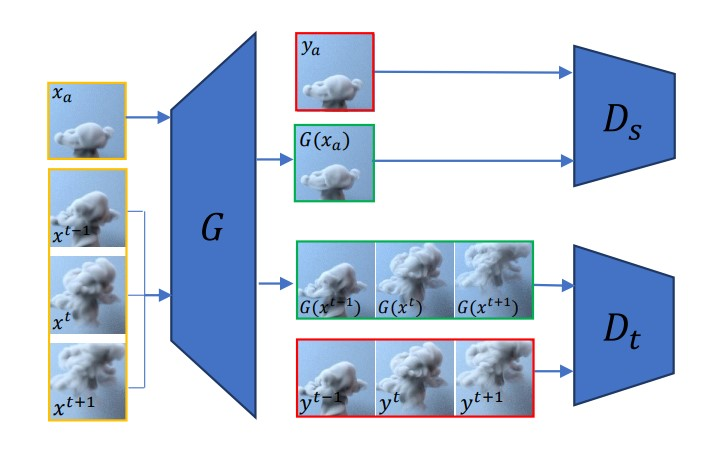
\includegraphics[width=11cm]{bilder/tempoGAN.jpg}
    \caption{Schematischer Aufbau des tempoGAN.}
    \source{\citet[95:2]{xie2018tempoGAN}}
    \label{tempoGAN-Aufbau}
\end{figure}

Das Netz dieser Arbeit hingegen nutzte jeweils nur einen Generator und Diskriminator während des Trainings. Ebenfalls wurden der Generator und Diskriminator jeweils mit einem Batch von 3D-Arrays trainiert. Ein Batch bestand aus mehreren Datenpaketen und jedes Paket erhielt drei temporal kohärente Frames einer Simulation. Jeder Frame, bestehend aus einem 3D-Array und wurde nochmals in kleinere, im Folgenden \textit{3D-Sub-Arrays} genannt, unterteilt. So hatte das ursprüngliche 3D-Array beispielsweise eine Auflösung von 192 $\cdot$ 192 $\cdot$ 192 Voxel und wurde anschließend in 27 kleinere 3D-Sub-Arrays mit der Auflösung 64 $\cdot$ 64 $\cdot$ 64 Voxel unterteilt. Das Training des Diskriminators bestand aus einem Batch mit zehn solcher 3D-Sub-Arrays. Anfängliche Tests zeigten, dass eine 1:1 Abbildung des tempoGAN-Netzes zu viel Speicherplatz innerhalb der Grafikkarte benötigte, weshalb es nicht möglich war, alle 27 3D-Sub-Arrays für das Training zu nutzen. Für den Generator wurden Low-Resolution-Versionen der 3D-Sub-Arrays erstellt. Die Auflösung dieser im Folgenden genannten \textit{LowRes-3D-Arrays} betrug 16 $\cdot$ 16 $\cdot$ 16 Voxel und wurde auf 64 $\cdot$ 64 $\cdot$ 64 Voxel hochskaliert, um die ursprüngliche Auflösung für den Input des Diskriminators zu erzeugen. Die tempoGAN-Implementierung nutzte hingegen alle 3D-Sub-Arrays eines Frames. Ebenso wurden weniger Convolutional und Residual Layer als im tempoGAN eingesetzt. Der Grund hierfür war, dass nur somit ein Training auf der Grafikkarte durchgeführt werden konnte. Deshalb wurde eine funktionierende Minimalvariante erstellt und trainiert. Im Folgenden werden die Architekturen des Generators und Diskriminators genauer beschrieben.

\subsection{Generator}
Es wurde eine höhere Anzahl an Convolutional und Residual Layer für den Generator, als für den Diskriminator gewählt, da dieser die komplexere Aufgabe des Upsamplings übernimmt. Die Architektur des Generators bestand aus einem anfänglichen Upsampling der Input-Daten und zwei lernfähigen Residual Blöcken. Die Upsampling Layer skalierten die Input-Daten auf die gewünschte Output-Größe. Es wurden ähnlich einer Transposed Convolution neue Voxel zwischen den bereits vorhandenen eingefügt. Diese neuen Voxel erhielten, basierend auf der \textit{Nearest Neighbor Interpolation}, denselben Wert, wie die am nächsten zu ihnen stehenden Nachbarn \parencite[]{nearestneighbor}. Anschließend wurden die Daten parallel durch die Residual Shortcut 1 und den Convolutional Block 1 geschleust. Letzterer enthielt doppelt so viele Convolutional Layer und erzeugte ebenso mehr Output Channels. Somit konnte das Netz mehr Feature Maps lernen und im besten Fall einen höheren Detailgrad in der Ausgabe erzeugen. Nachdem die Daten durch die beiden Blöcke geschleust wurden, konnten ihre Outputs summiert werden und dienten als Input für den nächsten Residual Block. Dort wurden die Daten wieder parallel in den die Residual Shortcut 2 und den Convolutional Block 2 gegeben und ihr Output anschließend summiert. Die Verfeinerung der Gewichte übernahm der ADAM Optimizer mit einer Lernrate von 0.0001. Es folgt eine grobe Übersicht über den Aufbau des Generators. Eine ausführliche Version findet sich im Anhang.
\newpage

\begin{enumerate}
    \item \underline{Input:} LowRes-3D-Array der Größe 16 $\cdot$ 16 $\cdot$ 16 Voxel mit 2 Input Channels (Density und Temperature)
    \item \underline{Upsample:} Ein Upsampling der 3D-Input-Daten zur Größe 32 $\cdot$ 32 $\cdot$ 32 Voxel.
    \item \underline{Upsample:} Ein Upsampling zur Größe 64 $\cdot$ 64 $\cdot$ 64 Voxel
    \item \underline{\textbf{Residual Block 1}} 
    \item[] \underline{Residual Shortcut 1} 
        \begin{enumerate}
            \item \underline{3D Convolutional Layer:} Input Channels 2, Output Channels 4
            \item \underline{3D BatchNorm:} Formt den Batch so, dass sein Durchschnittswert bei null und die Varianz bei eins liegt. Gilt für alle folgenden BatchNorm Layer.
        \end{enumerate}

    \item[] \underline{Convolutional Block 1}
        \begin{enumerate}
            \item \underline{3D Convolutional Layer:} Input Channels 2, Output Channels 4
            \item \underline{3D BatchNorm:}
            \item \underline{ReLU Aktivierungsfunktion:}
            \item \underline{3D Convolutional Layer:} Input Channels 2, Output Channels 4
            \item \underline{3D BatchNorm:}
        \end{enumerate}
        
    \item \underline{Summierter Output aus Residual-Shortcut 1 und Convolutional Block 1}
    \item \underline{\textbf{Residual Block 2}} 
    \item[] \underline{Residual Shortcut 2} 
        \begin{enumerate}
            \item \underline{3D Convolutional Layer:} Input Channels 4, Output Channels 2
            \item \underline{3D BatchNorm:}
        \end{enumerate}
    \item[] \underline{Convolutional Block 2}
        \begin{enumerate}
            \item \underline{3D Convolutional Layer:} Input Channels 4, Output Channels 8
            \item \underline{3D BatchNorm:}
            \item \underline{ReLU Aktivierungsfunktion:}
            \item \underline{3D Convolutional Layer:} Input Channels 8, Output Channels 2
            \item \underline{3D BatchNorm:}
        \end{enumerate}
    \item \underline{Summierter Output aus Residual Shortcut 2 und Convolutional Block 2}
    \item \underline{Output} 3D-Sub-Array der Größe 64 $\cdot$ 64 $\cdot$ 64 Voxel mit 2 Channels
\end{enumerate}

\subsection{Diskriminator}
Es folgt eine grobe Übersicht der Architektur des Diskriminators. Dieser wurde so aufgebaut, dass er dem temporalen Diskriminator der tempoGAN-Implementierung ähnelt. Als Input-Daten erhielt der Generator sechs Input Channels. Sie bestanden aus dem Density und Temperature Field eines Simulation-Frames. Insgesamt wurden drei aufeinanderfolgende Frames einer Simulation an den Input angelegt, um auf sechs Input Channels zu kommen. Jeder Channel bestand aus einem 3D-Sub-Array der Auflösung 64 $\cdot$ 64 $\cdot$ 64 Voxel. Über mehrere Convolutional Layer, einem Fully-Connected-Layer und einem einzelnen Output-Neuron lernte der Diskriminator den Input zu klassifizieren. Seine Ausgabe betrug 0,0, wenn er sich sicher war, dass die Input-Daten künstlich sind und 1,0, wenn er sie als echt klassifizierte. Zur Verfeinerung der Gewichte wurde ebenfalls der ADAM Optimizer mit einer Lernrate von 0.0001 eingesetzt. Eine ausführliche Version der Architektur findet sich ebenfalls im Anhang.

\begin{enumerate}
    \item \underline{Input} 3D-Sub-Array der Größe 64 $\cdot$ 64 $\cdot$ 64 Voxel mit 6 Input Channels (Density+Temperature für 3 Simulation-Frames)
    \item \underline{3D Convolutional Layer} Input Channels 6, Output Channels 8
    \item \underline{3D BatchNorm}
    \item \underline{Leaky-ReLU Aktivierungsfunktion} Eine Variante der normalen ReLU-Funktion, schneidet Werte im Minusbereich nicht ab \parencite[]{liu-2019}.
    \item \underline{3D Convolutional Layer} Input Channels 8, Output Channels 16
    \item \underline{3D BatchNorm}
    \item \underline{Leaky-ReLU Aktivierungsfunktion}
    \item \underline{3D Convolutional Layer} Input Channels 16, Output Channels 1
    \item \underline{Flatten} Wandelt alle dreidimensionalen Werte in einen eindimensionalen Layer an Neuronen um \parencite[]{meta-aiflatten}.
    \item \underline{Fully-Connected-Layer} Verbindet den eindimensionalen Layer an Neuronen mit dem letzten Neuron.
    \item \underline{Sigmoid-Aktivierungsfunktion} Erzeugt eine Ausgabe zwischen 0,0 und 1,0 \parencite[]{wood-2020}.
    \end{enumerate}


\section{Training des Netzes}
Im Folgenden wird die Trainingsschleife der beiden Netze erläutert. Die Daten entstammten dem in der Methodik beschriebenen Datensatz. Innerhalb einer Epoche wurden somit 5760 Frame-Pakete, zu sehen in Abbildung \ref{paket}, bestehend aus drei temporal kohärenten Frames mit Density und Temperature Fields verwendet. \\

\begin{figure}[ht]
    \centering
    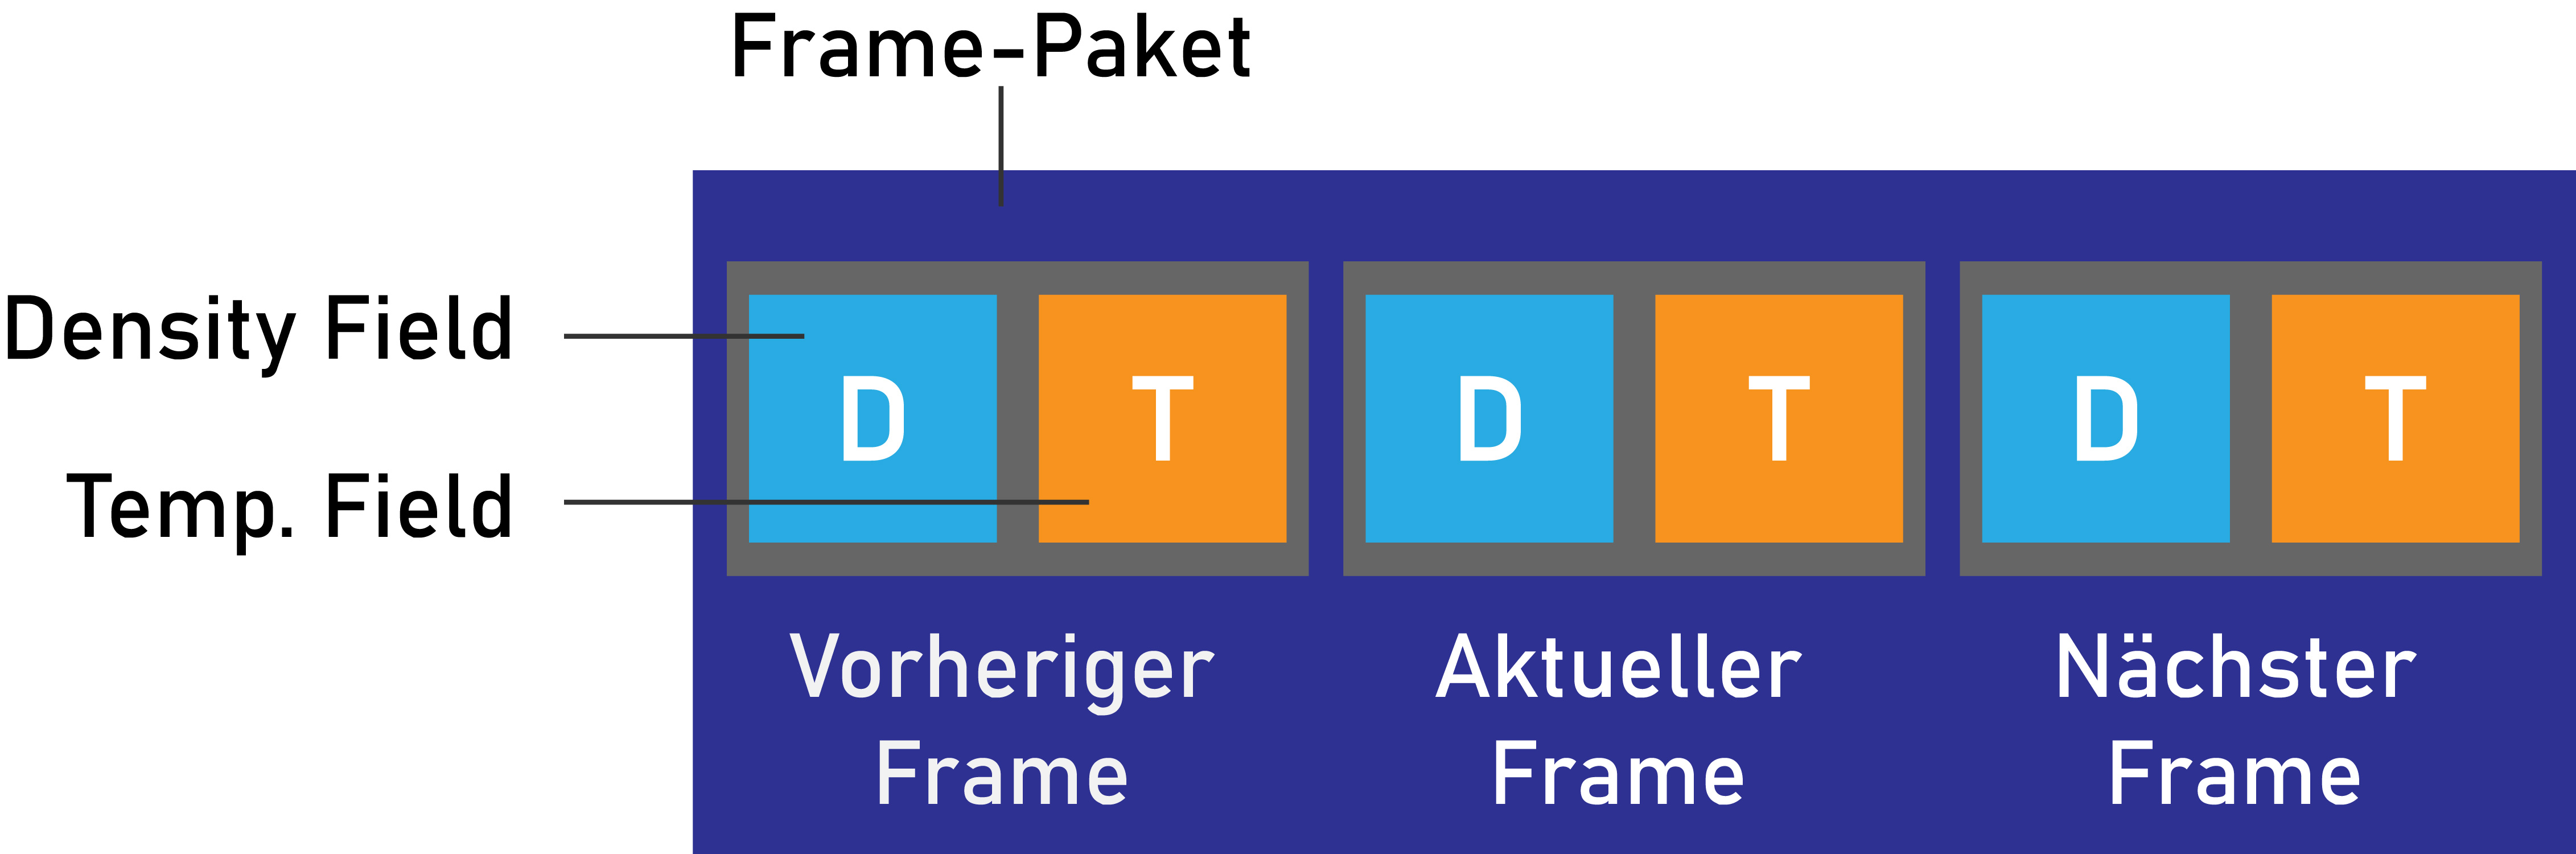
\includegraphics[width=11cm]{bilder/framepaket.jpg}
    \caption{Der Aufbau eines Frame-Pakets.}
    \source{Philipp Benner}
    \label{paket}
\end{figure}

Ein Batch enthielt zehn Frame-Pakete bestehend aus den Density und Temperature Fields des vorherigen, aktuellen und nächsten Frames. Jedes Field der Ursprungsgröße 192 $\cdot$ 192 $\cdot$ 192 Voxel wurde in 27 3D-Sub-Arrays der Größe 64 $\cdot$ 64 $\cdot$ 64 Voxel zerlegt (Abbildung \ref{fieldarray}). \\


\begin{figure}[ht]
    \centering
    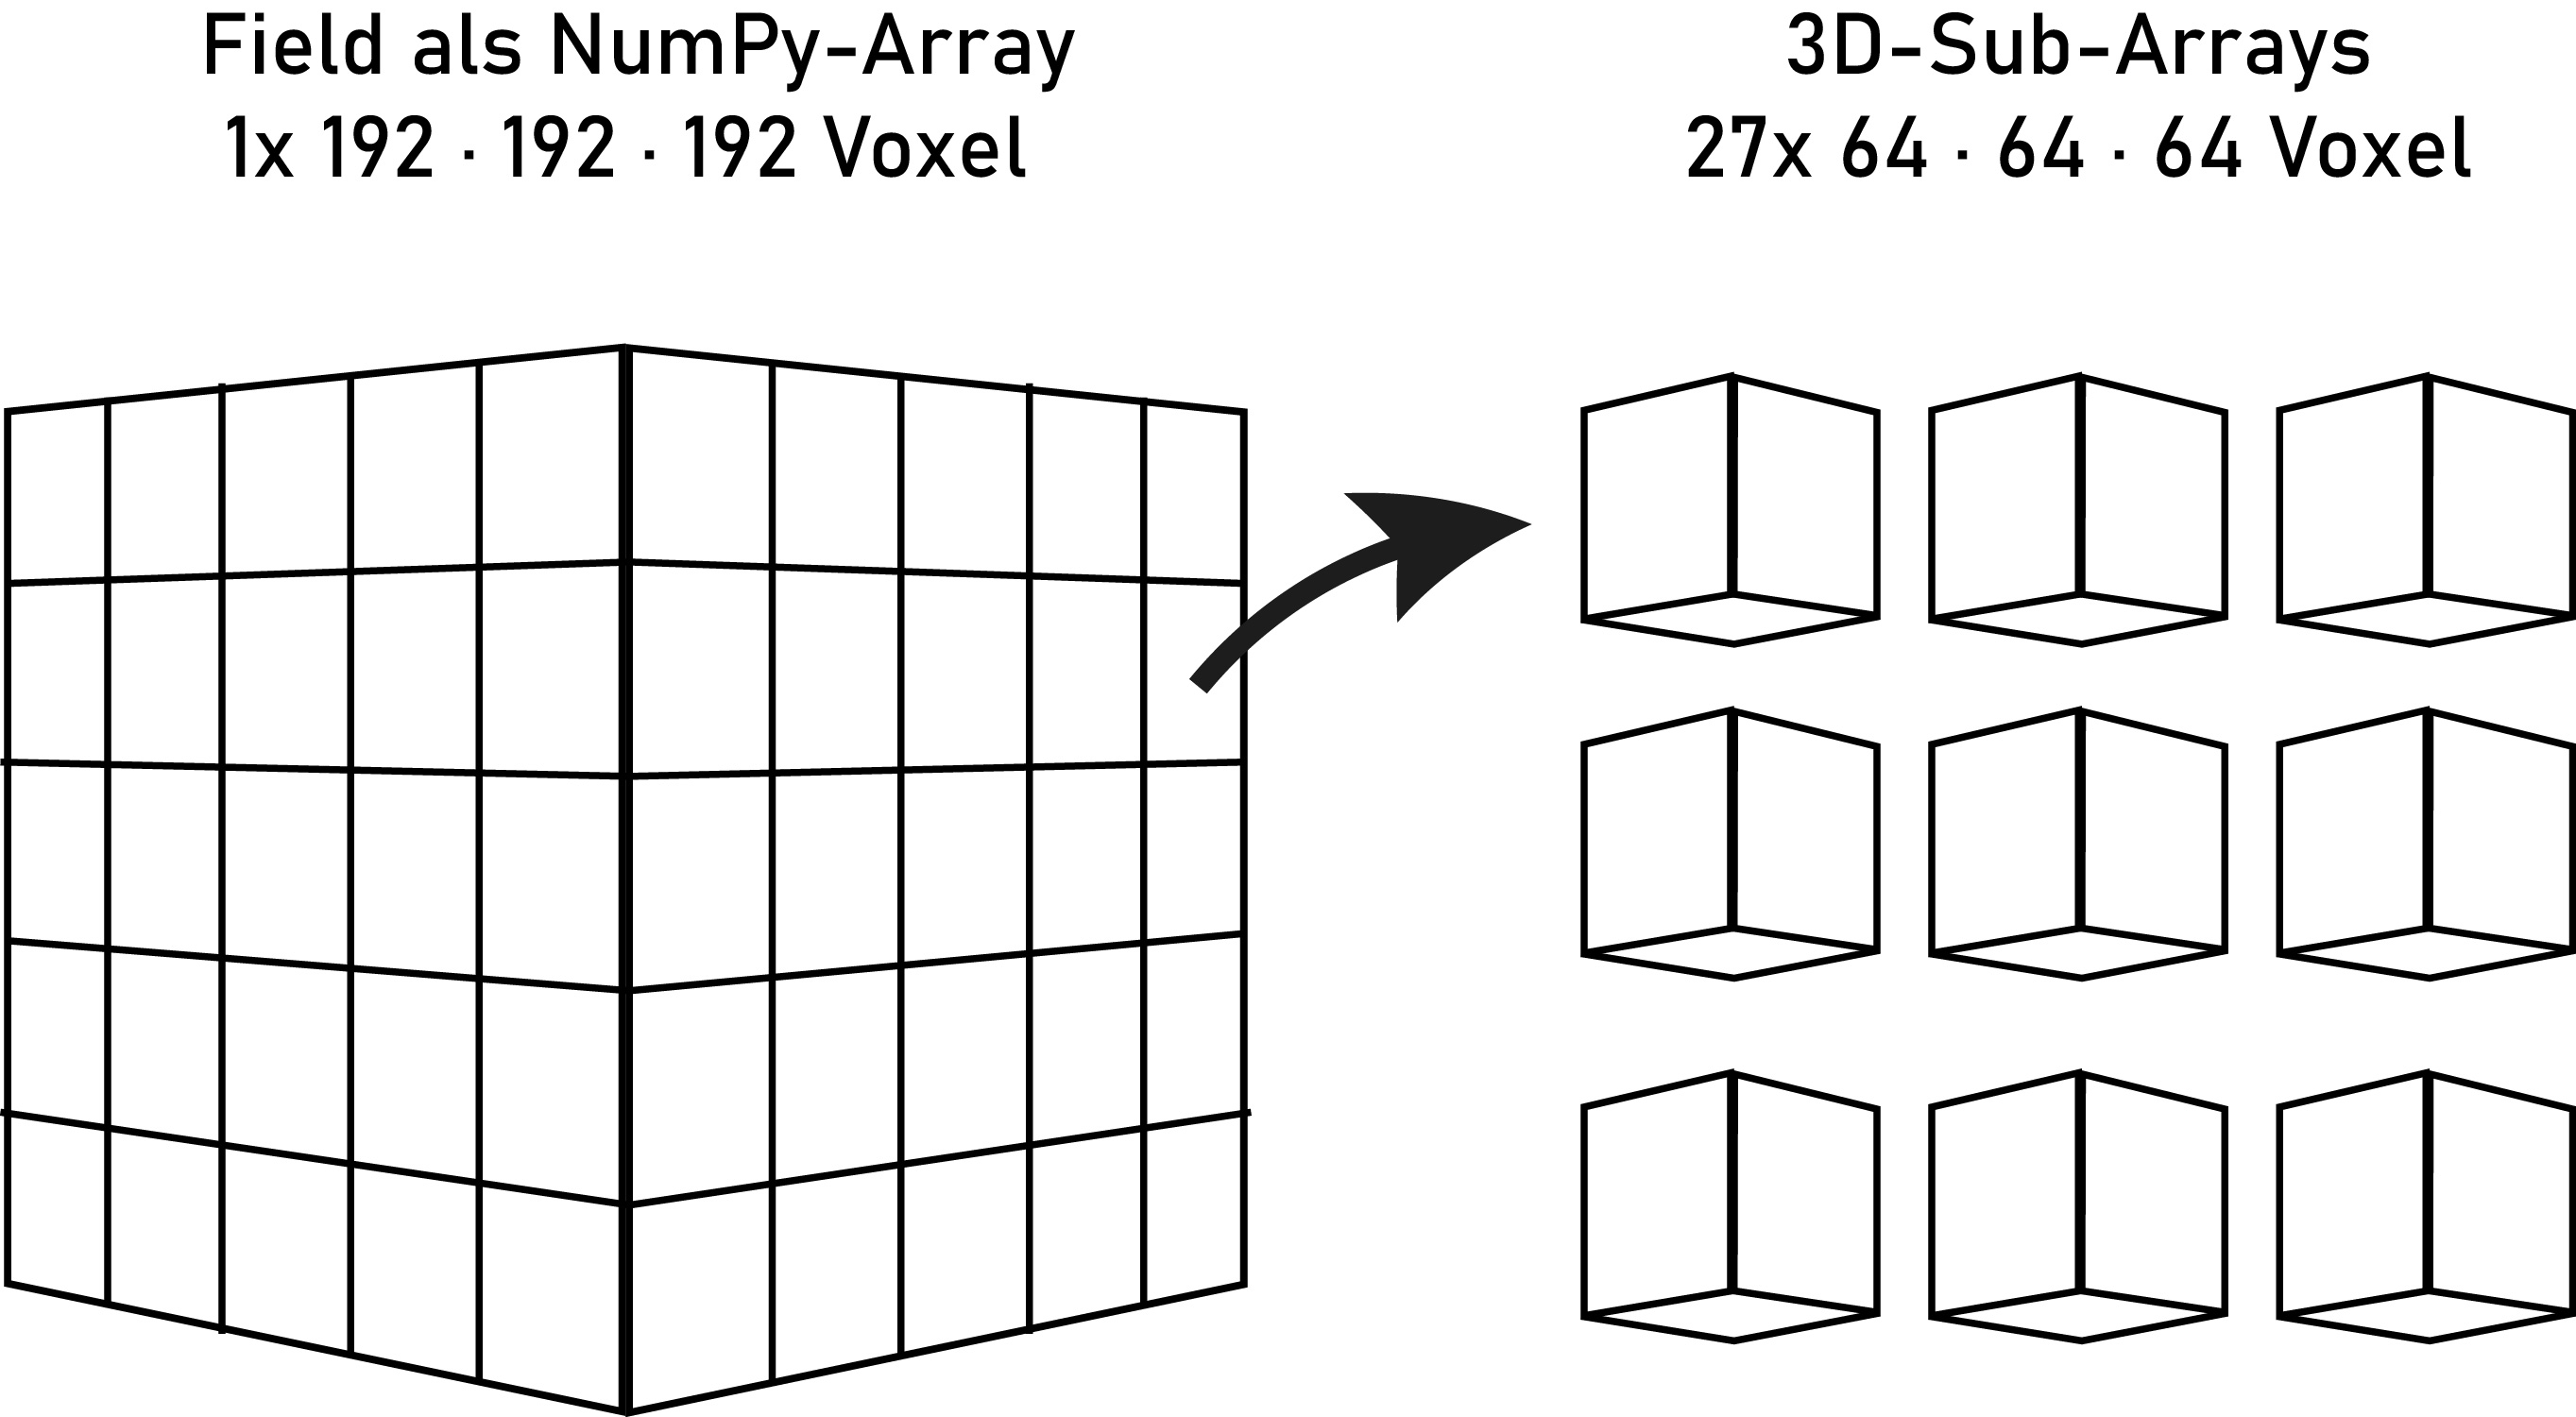
\includegraphics[width=11cm]{bilder/fieldarray.jpg}
    \caption{Umformung eines Fields in kleinere 3D-Sub-Arrays.}
    \source{Philipp Benner}
    \label{fieldarray}
\end{figure}


Somit ergab sich eine Anzahl von insgesamt 1620 einzelnen 3D-Sub-Arrays oder 810 Density und Temperature Paaren. Um auf der Grafikkarte trainieren zu können, konnten nicht alle 27 3D-Sub-Arrays eines Fields genutzt werden. Es wurden anstatt alle 27 Density und Temperature Field Paare eines Frames, nur jeweils ein Field-Paar pro Frame-Paket genutzt. Eine zufällige Selektion wählte  zehn Frame-Pakete mit jeweils sechs 3D-Sub-Arrays bestehend aus den drei aufeinanderfolgenden Frames und deren Fields aus. Ein Batch enthielt somit 10 Frame-Pakete bestehend aus sechs 3D-Sub-Arrays der Frames und deren Fields, insgesamt 60 3D-Sub-Arrays oder 30 Field-Paare aus temporal kohärenten Frames. Die sechs 3D-Sub-Arrays wurden als Input-Daten für die Convolutional Layer der beiden Netzwerke genutzt. Hierbei entstand ein weiterer Unterschied zur tempoGAN-Implementierung. In dessen Implementierung wurden alle 3D-Sub-Arrays für das Training genutzt und somit konnte ein kompletter Frame durch den Diskriminator und den Generator geschleust werden. In dieser Implementierung hingegen konnte nur der Teil eines Frames durch das Netz geschleust werden.\\

Das Training begann mit echten Daten im Diskriminator und es wurde diesem mitgeteilt, dass die Klassifizierung 1,0 betragen solle. Dazu wurde der Batch durch den Diskriminator geleitet, dessen Fehlerwert berechnet und anschließend die Gewichte aktualisiert.\\

Danach begann das Training des Diskriminators auf Daten trainiert, deren Label 0,0 betrug. Dazu wurde ein neuer Batch mit denselben Dimensionen der LowRes-3D-Arrays basierend auf Noise erzeugt, um falsche Daten zu erzeugen. Der Generator skalierte diesen Batch im Anschluss auf eine höhere Auflösung und er durchlief danach den Diskriminator, der den Bach mit dem Wert 0,0 klassifizierte. Der Fehlerwert wurde berechnet und anschließend die Gewichte aktualisiert.\\

Da der Generator nicht mit sechs Input Channels von aufeinanderfolgenden Frames trainiert werden sollte, sondern nur mit zwei, musste der Batch vor dem Training des Generators umgeformt werden. Der Grund hierfür war, dass es bei einer späteren Implementierung in einer VFX Software möglich sein soll, einen einzelnen Frame anhand des Density und Temperature Fields in seiner Auflösung zu skalieren. Dabei sollen der vorherige und nächste Frame nicht berücksichtigt werden. Der bestehende Batch echter Daten wurde aufgebrochen und in sechs kleinere Batches unterteilt. Somit konnte aus jedem Frame-Paket jeweils ein einzelner Batch pro Frame erzeugt werden. Jeder Batch enthielt nun zwei 3D-Sub-Arrays mit jeweils einem Field. Es wurden anschließend anstatt ein Batch mit mehreren Frame-Paketen, einzelne Frames durch den Generator geschleust. Der Generator erzeugte aus zwei LowRes-3D-Arrays der Größe 16 $\cdot$ 16 $\cdot$ 16 einen Output aus zwei Arrays der Größe 64 $\cdot$ 64 $\cdot$ 64. Die sechs Paare der hochskalierten Arrays wurden nun wieder in einem Batch gebündelt, der die ursprüngliche Batch-Form besitzt. Dieser Batch durchlief den Diskriminator geschleust und mit dem Fehlerwert des Diskriminators wurden die Gewichte des Generators aktualisiert. \\

Es wurden vor jedem aktualisieren der Gewichte, der aktuelle Fehlerwert für die beiden Durchgänge des Diskriminators und den des Generators gespeichert, um die Genauigkeit des Netzes evaluieren zu können.\\

Das Netz konnte während des Trainings nicht mit Testdaten getestet werden, da nicht ausreichend Speicher innerhalb der Grafikkarte für diese Daten zur Verfügung stand.\\

\section{Ausgabe des Netzes}
Nach dem Training des Netzes, war es in der Lage zwei Input-Arrays der Größe 16 $\cdot$ 16 $\cdot$ 16 auf die Größe 64 $\cdot$ 64 $\cdot$ 64 zu skalieren. Dies entspricht einem Faktor von vier für jede Dimension und 64 Mal mehr Voxel insgesamt. Um einen kompletten Frame einer Simulation im OpenVDB Format mithilfe der KI zu skalieren, musste der Frame mittels des Python-Skripts in ein 3D-NumPy-Array konvertiert und anschließend in einzelne 3D-Sub-Arrays aufgeteilt werden. Nach dem Konvertieren der 3D-Sub-Arrays in LowRes-3D-Arrays wurden diese durch den Generator schleust und er erzeugte eine skalierte Version. Anschließend durchliefen die einzelnen 3D-Sub-Arrays eine Umformung zu einem großen Array und es folgte eine Konvertierung zurück ins OpenVDB Format. 